%%
%% CSD (CSL559) - OpenTelemetry assignment report
%% Same ACM "acmart" manuscript style as the Assignment 1 report.
%%
\documentclass[manuscript,screen]{acmart}

\usepackage{tikz}
\usetikzlibrary{arrows.meta,positioning,fit}
\usepackage{listings}
\usepackage{booktabs}
\usepackage{array}
\usepackage{placeins}

\lstset{
  basicstyle=\ttfamily\footnotesize,
  breaklines=true,
  columns=fullflexible,
  frame=single,
  framerule=0.3pt,
  rulecolor=\color{gray!50},
  backgroundcolor=\color{gray!5},
  showstringspaces=false,
}

\AtBeginDocument{\providecommand\BibTeX{{Bib\TeX}}}
\settopmatter{printacmref=false}
\setcopyright{none}
\renewcommand\footnotetextcopyrightpermission[1]{}
\pagestyle{plain}

\begin{document}
\sloppy

\title{Observing the Village Pond Planning System with OpenTelemetry}
\subtitle{CSL559 System Design -- OpenTelemetry Assignment (Assignment~1, Phase~3)}

\author{Your Full Name}
\affiliation{%
  \institution{Your Institute / Department}
  \city{Your City}
  \country{India}}
\email{your.email@institute.ac.in}

\renewcommand{\shortauthors}{Your Surname}

\begin{abstract}
We added OpenTelemetry to our Assignment~1 project, the AI-based Village
Pond Planning System, which is deployed at \url{http://10.1.75.51:3305}.
The FastAPI backend and the React frontend now produce
\emph{traces}, \emph{metrics} and \emph{logs}. They send them over OTLP
to an OpenTelemetry Collector on a second course container, and the
Collector forwards them to OpenObserve, an open-source backend that stores
all three signals and shows them in a web UI at \url{http://10.1.75.51:3306}.
A single trace follows one analysis from the user's click in the browser,
through every stage of the backend pipeline, to the three external APIs it
calls (AWS elevation tiles, NASA POWER, Open-Meteo). Every screenshot in
this report comes from the running deployment. The telemetry answered real
questions about the system:
\begin{itemize}
\item a 15.4~s request spent 11.1~s waiting behind other users;
\item on a warm cache, CPU-bound hydrology, not downloading, is the cost;
\item the two rainfall sources win the race almost equally often (30 vs.\ 26 lookups);
\item the observability backend was dropping data, and we found out why.
\end{itemize}
\end{abstract}

\keywords{OpenTelemetry, Observability, Distributed Tracing, Metrics,
Logging, OTLP, OpenObserve}

\maketitle

%% =====================================================================
\section{Why the pond planner needs observability}
\label{sec:why}

The pond planner takes a polygon drawn on a map (or a KML contour file) and
returns the best pond sites, their catchments and the water each can
collect. One request does the following:
\begin{itemize}
\item downloads elevation tiles from AWS;
\item queries two rainfall services;
\item fills sinks, routes flow (D8) and accumulates it over a grid of up to
  250{,}000 cells;
\item ranks candidate sites and delineates each catchment.
\end{itemize}
All of this runs in one 512~MB, 1~vCPU container that allows a single
analysis at a time.

Before this assignment, the only window into the running system was the
Uvicorn access log, for example
\texttt{"POST /api/analyze-area HTTP/1.1" 200}. When a user reported that an
analysis ``took 15 seconds'', that line could not tell us whether the time
went on the network, on the CPU, or on waiting behind someone else. As
the lecture put it, \emph{in production the only thing you can see is what
the system tells you}. The goal of this work is to make the system tell us
enough to answer such questions without attaching a debugger.

%% =====================================================================
\section{Architecture}
\label{sec:architecture}

Figure~\ref{fig:architecture} shows the deployment. It follows the
\emph{instrument $\rightarrow$ collect $\rightarrow$ store and view} model
from the lecture. Each step runs as its own process, and the application
code never names the storage backend.

\begin{figure}[htbp]
\centering
\resizebox{\linewidth}{!}{%
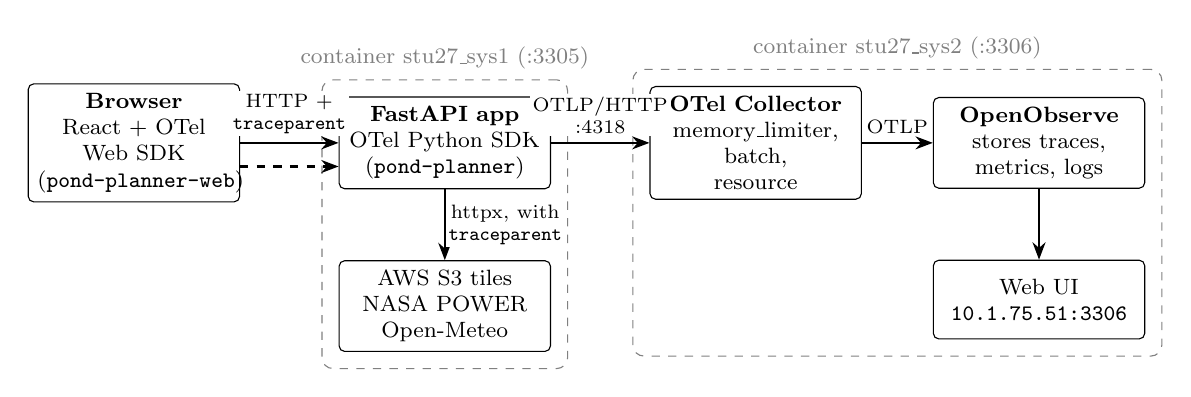
\begin{tikzpicture}[
  font=\footnotesize,
  box/.style={draw, rounded corners=2pt, align=center, minimum height=1.0cm,
              text width=2.45cm, fill=white},
  host/.style={draw, dashed, rounded corners=4pt, inner sep=6pt, gray},
  arr/.style={-{Stealth[length=2.2mm]}, thick},
  lbl/.style={font=\scriptsize, align=center, fill=white, inner sep=1pt}]
  \node[box] (browser) {\textbf{Browser}\\React + OTel Web SDK\\(\texttt{pond-planner-web})};
  \node[box, right=1.25cm of browser] (app) {\textbf{FastAPI app}\\OTel Python SDK\\(\texttt{pond-planner})};
  \node[box, below=0.9cm of app] (ext) {AWS S3 tiles\\NASA POWER\\Open-Meteo};
  \node[box, right=1.25cm of app] (col) {\textbf{OTel Collector}\\memory\_limiter, batch,\\resource};
  \node[box, right=0.9cm of col] (oo) {\textbf{OpenObserve}\\stores traces,\\metrics, logs};
  \node[box, below=0.9cm of oo] (ui) {Web UI\\\texttt{10.1.75.51:3306}};
  \node[host, fit=(app)(ext), label={[gray]above:{container stu27\_sys1 (:3305)}}] {};
  \node[host, fit=(col)(oo)(ui), label={[gray]above:{container stu27\_sys2 (:3306)}}] {};
  \draw[arr] (browser) -- node[lbl, above=2pt] {HTTP +\\\texttt{traceparent}} (app);
  \draw[arr, dashed] ([yshift=-3mm]browser.east) -- ([yshift=-3mm]app.west);
  \draw[arr] (app) -- node[lbl, right] {httpx, with\\\texttt{traceparent}} (ext);
  \draw[arr] (app) -- node[lbl, above=2pt] {OTLP/HTTP\\:4318} (col);
  \draw[arr] (col) -- node[lbl, above=2pt] {OTLP} (oo);
  \draw[arr] (oo) -- (ui);
\end{tikzpicture}}
\caption{Deployment. Solid arrows carry requests or telemetry. The dashed
arrow shows the browser's spans, which travel via the app's
\texttt{/otel/v1/traces} endpoint because the browser can only reach port
3305. The Collector listens only on the internal Docker network
(172.17.0.107); only the OpenObserve UI is published.}
\label{fig:architecture}
\end{figure}

\paragraph{Why two containers.} OpenObserve needs about 270--330~MB of
memory. The app container already uses about 280~MB at peak (Assignment~1
measurements) out of its 512~MB, so both cannot share it. The course
provides four containers, so the Collector and OpenObserve run on a
second one (\texttt{stu27\_sys2}). The two containers reach each other over
Docker's internal network.

\paragraph{Why a Collector at all.} The app could send directly to
OpenObserve. Putting a Collector in between has two benefits:
\begin{itemize}
\item \emph{Decoupling.} Changing or adding a backend (Jaeger, Prometheus,
  Grafana) is an edit to one YAML file. The app does not change.
\item \emph{Buffering.} The Collector batches data and retries failed
  sends, so a backend outage does not slow the app. Section~\ref{sec:lessons}
  shows this mattered.
\end{itemize}

%% =====================================================================
\section{Implementation}
\label{sec:implementation}

\subsection{Backend: automatic instrumentation}
All set-up lives in one module, \texttt{backend/app/telemetry.py}. It is
called before the routes are imported, so that the services' HTTP clients
are already instrumented when they are created. Four instrumentations
need no changes to the application code:
\begin{itemize}
\item \textbf{FastAPI}: a server span and request-duration metrics for every
  API call. Health checks and static files are excluded, as are the
  per-chunk ASGI send/receive spans; a 6.4~MB upload produced 517 of those
  before we excluded them.
\item \textbf{httpx}: a client span for every outgoing call (each tile and
  each rainfall request). It also injects the W3C \texttt{traceparent}
  header into those calls.
\item \textbf{System metrics}: process memory, CPU, thread count and garbage
  collection, important on a 512~MB host.
\item \textbf{Logging}: an OTLP log handler on the root logger, so every
  existing \texttt{logging} call is exported with the trace and span ID of
  the request that produced it.
\end{itemize}

\subsection{Backend: manual spans}
Automatic spans show only the HTTP edges. To see \emph{inside} an analysis
we wrapped each pipeline stage in a span (Table~\ref{tab:spans}), using the
API from the lecture slides:

\begin{lstlisting}[language=Python]
with tracer.start_as_current_span("terrain.build") as span:
    terrain, dem_info = build_terrain_from_polygon(polygon)
    span.set_attribute("pond.tiles.count", tile_count)
\end{lstlisting}

\begin{table}[h]
\caption{Manual spans added to the backend}
\label{tab:spans}
\small
\begin{tabular}{>{\raggedright\arraybackslash}p{5.2cm}>{\raggedright\arraybackslash}p{8.6cm}}
\toprule
Span & What it covers (key attributes) \\
\midrule
\texttt{queue.wait} & Waiting for the single processing slot (\texttt{pond.queue.wait\_s}) \\
\texttt{terrain.build} & Polygon $\rightarrow$ elevation grid (\texttt{pond.area\_km2}, \texttt{pond.grid.cells}, \texttt{pond.tiles.zoom}, \texttt{pond.tiles.count}) \\
\texttt{tiles.download} & Fetching missing tiles (\texttt{pond.tiles.needed/cached/missing}) \\
\texttt{tiles.decode\_and\_stitch} & PNG decode and mosaic \\
\texttt{rainfall.lookup} & Cache check and source race (\texttt{pond.rainfall.cache\_hit}, \texttt{pond.rainfall.source}) \\
\texttt{rainfall.nasa\_power}, \texttt{rainfall.open\_meteo} & One span per rainfall source; both run in parallel \\
\texttt{rainfall.wait} & Time the pipeline waited for the background rainfall lookup \\
\texttt{hydrology.fill\_sinks\_and\_d8} & Sink filling and D8 flow direction (\texttt{pond.flow.filled\_cells}) \\
\texttt{hydrology.flow\_accumulation} & Flow accumulation \\
\texttt{hydrology.rank\_pond\_sites} & Site scoring and selection (\texttt{pond.candidates.found}) \\
\texttt{hydrology.catchments\_and\_volume} & Catchment delineation and runoff volume per site \\
\texttt{contours.generate}, \texttt{kml.parse}, \texttt{terrain.reconstruct\_from\_contours} & Contour display, KML parsing, contour-to-grid interpolation \\
\bottomrule
\end{tabular}
\end{table}

\paragraph{Keeping one trace across threads.} The backend runs heavy work
in worker threads: the analysis itself, eight parallel tile loads, and the
two rainfall sources racing each other. Python's
\texttt{ThreadPoolExecutor} does not carry the OpenTelemetry context into
its threads, so our first version produced a separate, parentless trace
for each rainfall lookup. We fixed this with a small wrapper that
re-attaches the caller's context in the worker:

\begin{lstlisting}[language=Python]
def in_current_context(func):
    parent = otel_context.get_current()
    def run(*args, **kwargs):
        token = otel_context.attach(parent)
        try:
            return func(*args, **kwargs)
        finally:
            otel_context.detach(token)
    return run
\end{lstlisting}

With it, one request produces one trace of about 20--25 spans, with
correct parent--child links (verified with an in-memory exporter before
deployment).

\subsection{Backend: custom metrics}
Spans describe single requests. Metrics aggregate across all of them
cheaply. We added the metrics in Table~\ref{tab:metrics}, recorded at the
same points as the spans.

\begin{table}[h]
\caption{Custom metrics (meter \texttt{pond.planner})}
\label{tab:metrics}
\small
\begin{tabular}{>{\raggedright\arraybackslash}p{4.6cm}>{\raggedright\arraybackslash}p{2.3cm}>{\raggedright\arraybackslash}p{6.9cm}}
\toprule
Metric & Type & Attributes / purpose \\
\midrule
\texttt{pond.analysis.count} & Counter & \texttt{mode} (area/contour), \texttt{outcome} (success, invalid\_area, bad\_file\_type, \ldots) \\
\texttt{pond.analysis.duration} & Histogram (s) & End-to-end analysis time \\
\texttt{pond.analysis.stage.duration} & Histogram (s) & \texttt{stage}: time per pipeline stage \\
\texttt{pond.queue.wait} & Histogram (s) & Waiting for the processing slot \\
\texttt{pond.analyses.active} & UpDownCounter & Analyses running or queued \\
\texttt{pond.tiles.requests} & Counter & \texttt{result}: cache\_hit, downloaded, failed \\
\texttt{pond.rainfall.lookups} & Counter & \texttt{source}: cache, NASA POWER, Open-Meteo, fallback, user\_supplied \\
\texttt{pond.candidates.found}, \texttt{pond.grid.cells}, \texttt{pond.area.size}, \texttt{pond.best\_site.annual\_runoff} & Histograms & Size of the work and of the answer \\
\bottomrule
\end{tabular}
\end{table}

\paragraph{Histogram buckets.} The SDK's default histogram buckets
(0, 5, 10, 25, \ldots) are designed for milliseconds. Our durations are
recorded in seconds, so almost every analysis fell into the first
``0--5'' bucket, and every stage reported the same meaningless p95 of
4.75~s. We noticed this on the first dashboard and set explicit bucket
boundaries per metric (for seconds: 0.01 to 120). It is a reminder that a
metric is only as good as its aggregation.

\subsection{Frontend: browser tracing}
The React app uses the OpenTelemetry Web SDK with two instrumentations:
\begin{itemize}
\item \emph{document-load}: page-load timing;
\item \emph{fetch}: a span for each API call, which also adds a
  \texttt{traceparent} header to it.
\end{itemize}
Each analysis is wrapped in a \texttt{ui.analyze\_area} (or
\texttt{ui.analyze\_contour\_file}) span. The backend reads the incoming
\texttt{traceparent} header, so its server span becomes a child of the
browser's span, and the whole request appears as \emph{one} trace across
two services. This is the ``give every request an ID and pass it on''
idea from the lecture, standardised as W3C Trace Context.

The browser cannot reach the Collector, which is internal, so it posts its
spans to \texttt{/otel/v1/traces} on the app. The app forwards them
unchanged and does not trace this forwarding, to avoid a feedback loop.

\subsection{Collector and backend configuration}
The Collector (core distribution, v0.162.0) has one pipeline per signal:
\begin{itemize}
\item an \texttt{otlp} receiver;
\item three processors: \texttt{memory\_limiter} (refuses data before the
  container runs out of memory), \texttt{batch} (one HTTP call per batch
  rather than per span) and \texttt{resource} (tags data with
  \texttt{collector.host});
\item two exporters: \texttt{otlp\_http} to OpenObserve, and
  \texttt{debug}, which logs a one-line summary of each batch.
\end{itemize}
An excerpt of that summary log:
\begin{lstlisting}
2026-10-16 16:50:43 Logs    resource logs=2 log records=2
2026-10-16 16:50:48 Traces  resource spans=1 spans=13
2026-10-16 16:50:50 Metrics resource metrics=1 metrics=25 data points=536
\end{lstlisting}

The app is configured only through standard environment variables
(\texttt{OTEL\_SERVICE\_NAME}, \texttt{OTEL\_EXPORTER\_OTLP\_ENDPOINT}).
The same code runs locally with no exporter: spans are still created, and
trace IDs still appear in the console log.

%% =====================================================================
\section{Tools, libraries and services}
\label{sec:tools}

\begin{table}[h]
\caption{Components used}
\label{tab:tools}
\small
\begin{tabular}{>{\raggedright\arraybackslash}p{5.6cm}>{\raggedright\arraybackslash}p{2.9cm}>{\raggedright\arraybackslash}p{5.3cm}}
\toprule
Component & Version & Role \\
\midrule
\texttt{opentelemetry-api}, \texttt{-sdk} (Python) & 1.45.1 & API and SDK in the backend \\
\texttt{opentelemetry-exporter-otlp-proto-http} & 1.45.1 & OTLP/HTTP export of traces, metrics, logs \\
\texttt{opentelemetry-instrumentation-fastapi}, \texttt{-httpx} & 0.66b1 & Automatic server and client spans \\
\texttt{opentelemetry-instrumentation-logging}, \texttt{-system-metrics} & 0.66b1 & Log export, process metrics \\
\texttt{@opentelemetry/sdk-trace-web} (+ fetch, document-load) & 2.12 / 0.223 & Browser tracing \\
OpenTelemetry Collector (core) & 0.162.0 & Receive, batch, limit memory, export \\
OpenObserve & 1.0.0 & Storage and UI for all three signals \\
Pond Planner backend & FastAPI 0.141, Python 3.14 & The instrumented application \\
Course containers & Ubuntu 24.04, 512 MB, 1 vCPU & sys1: app; sys2: Collector + OpenObserve \\
\bottomrule
\end{tabular}
\end{table}

We chose OpenObserve over the common Jaeger + Prometheus + Loki + Grafana
stack because it is a single binary that stores and displays traces,
metrics and logs together, which fits on one 512~MB container. Because the
app speaks plain OTLP, switching to that stack later would only change the
Collector's exporter section.

%% =====================================================================
\section{Results: what the screenshots show}
\label{sec:results}

All screenshots were taken from the running deployment on 16~October~2026.
The traffic was a mix of real browser sessions and scripted requests: areas
at ten Indian locations (1--25~km$^2$), one 6.4~MB contour upload,
deliberately invalid inputs, and four simultaneous large requests. In about
40 minutes the system recorded 876 spans in 106 traces and 212 log records,
plus 81 metric streams.

\subsection{The application being observed}

\begin{figure}[htbp]
  \centering
  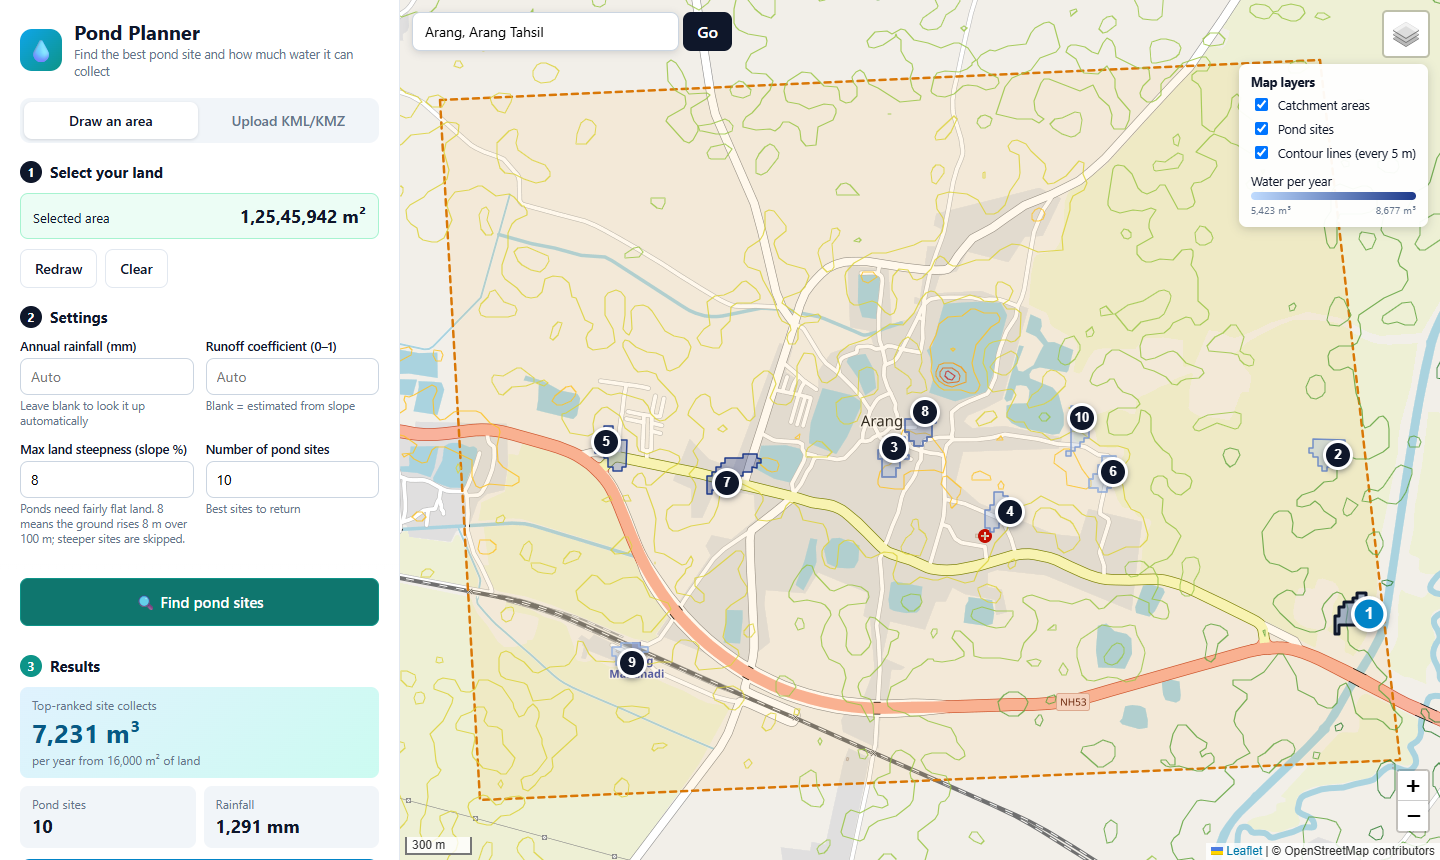
\includegraphics[width=0.85\linewidth]{figures/01_app_result}
  \caption{The pond planner at \texttt{10.1.75.51:3305} after a user drew a
  12.5~km$^2$ area around Arang (Chhattisgarh) and clicked \emph{Find pond
  sites}: ten ranked sites, their catchments and contour lines. This click
  produced the trace in Figure~\ref{fig:waterfall}.}
  \label{fig:app}
\end{figure}

\FloatBarrier
\subsection{Traces}

\begin{figure}[htbp]
  \centering
  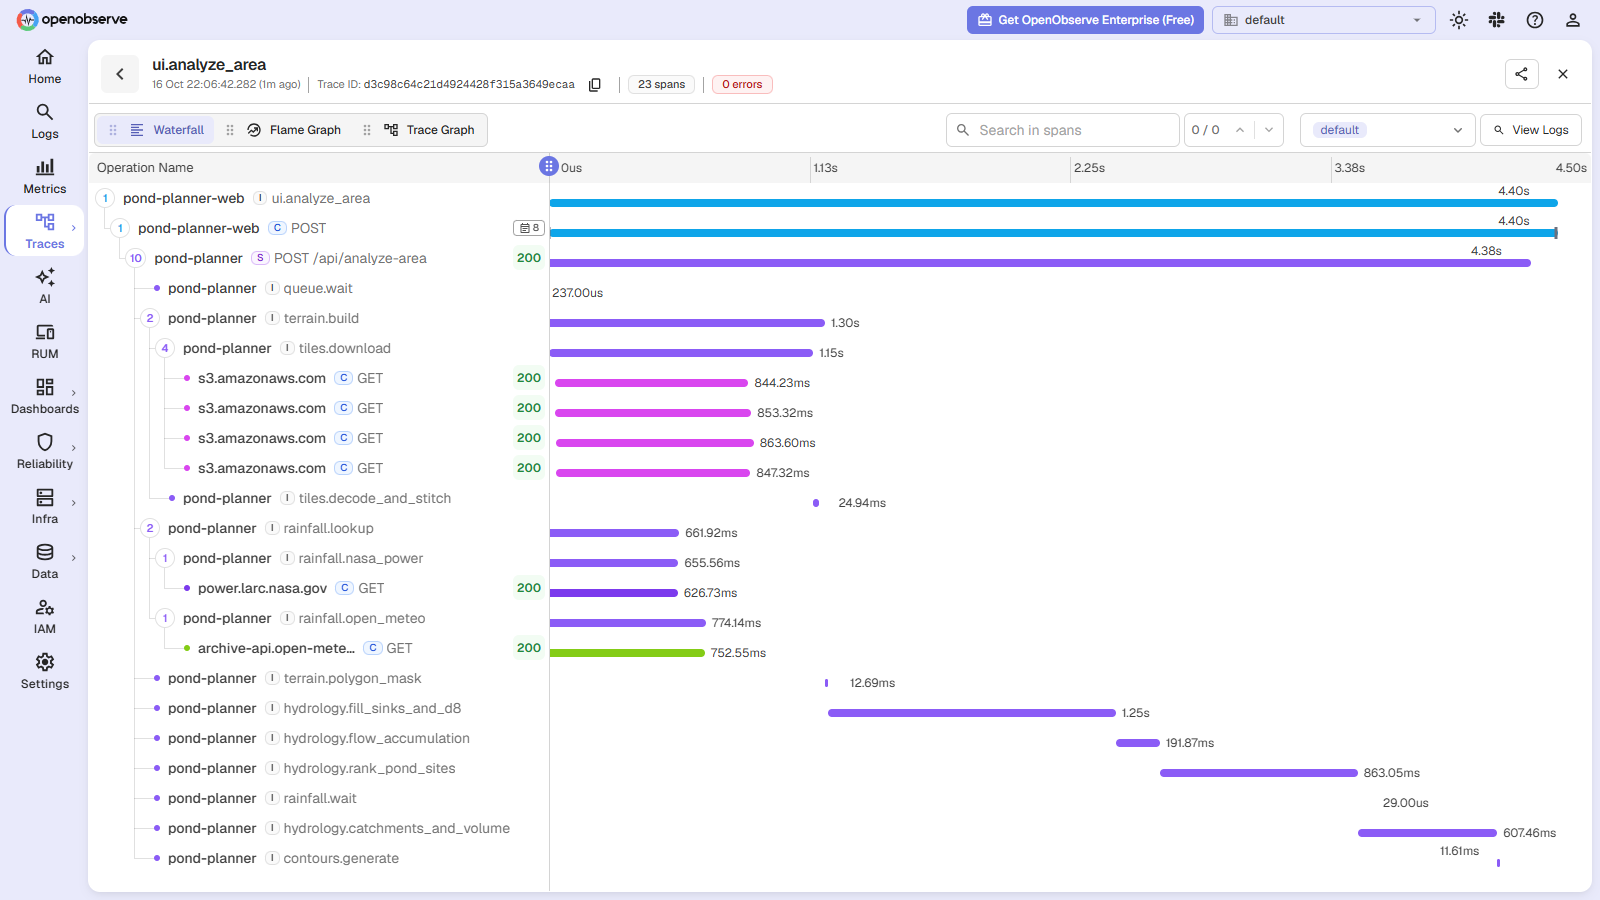
\includegraphics[width=\linewidth]{figures/02_trace_waterfall_browser_to_backend}
  \caption{\textbf{One request, end to end (waterfall view).} Trace
  \texttt{d3c98c64\ldots} has 23 spans from two services:
  \texttt{pond-planner-web} (browser, top two rows) and
  \texttt{pond-planner} (backend). The user waited 4.40~s. Tile download took about 1.15~s (four
  parallel \texttt{GET}s to \texttt{s3.amazonaws.com}, 844--864~ms each).
  The rainfall race, NASA POWER (656~ms) against Open-Meteo (774~ms), ran
  at the same time as the tile download, so it added nothing to the total.
  Then came sink filling and D8 (1.25~s), site ranking (0.86~s), and
  catchments and volumes (0.61~s). \texttt{rainfall.wait} is 29~$\mu$s: rainfall was ready long before the
  pipeline needed it, which confirms the overlap design from
  Assignment~1.}
  \label{fig:waterfall}
\end{figure}

\begin{figure}[htbp]
  \centering
  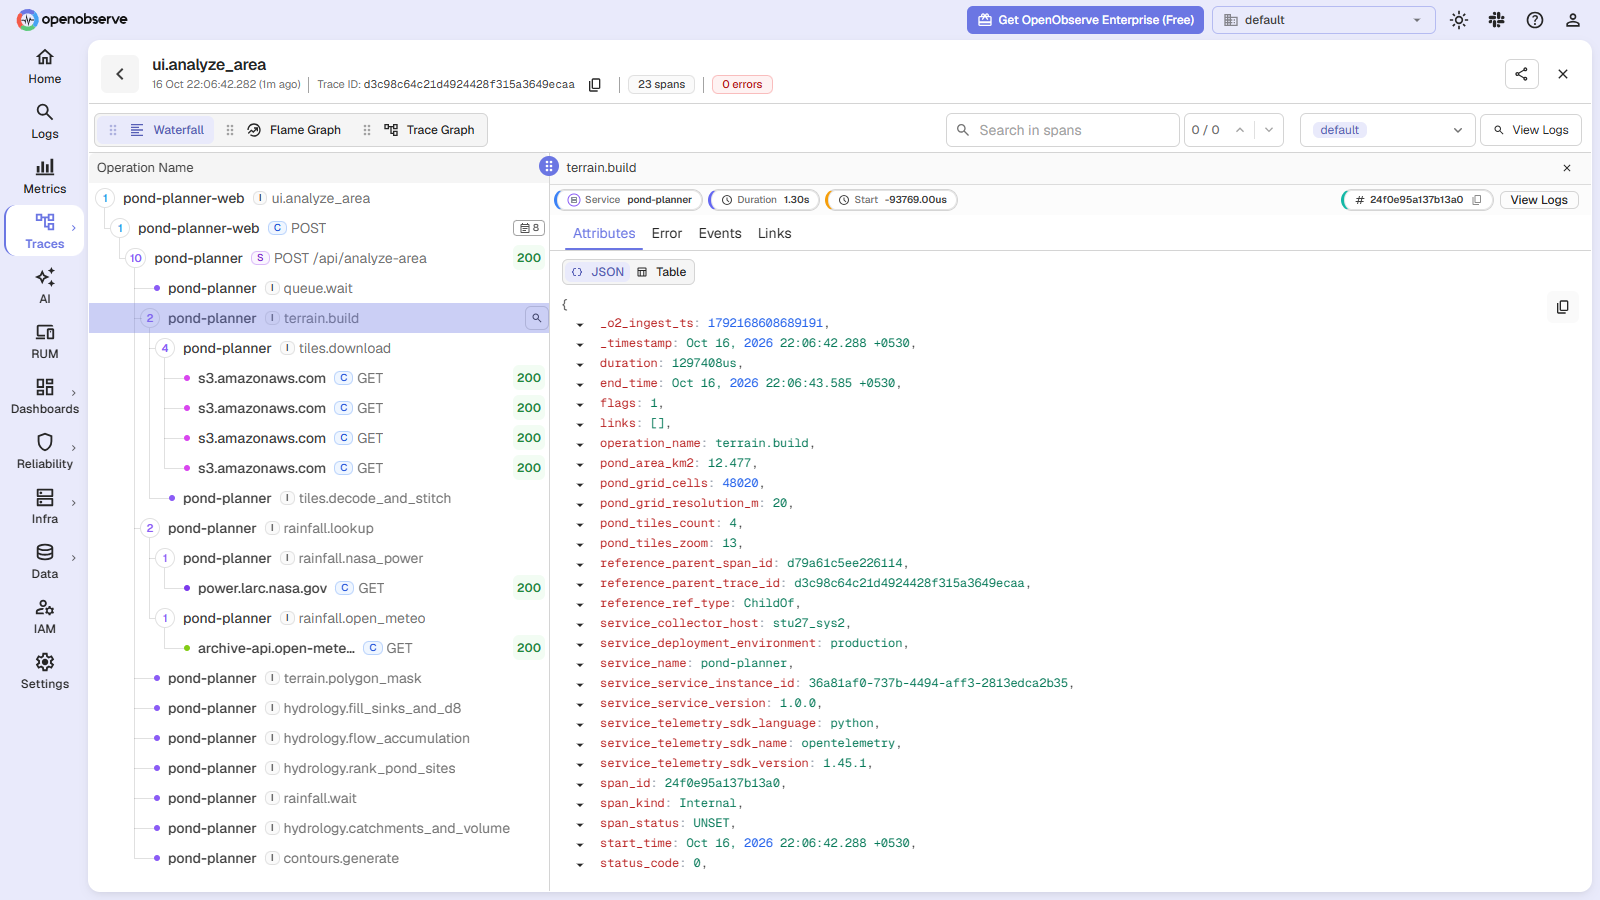
\includegraphics[width=\linewidth]{figures/03_span_attributes}
  \caption{\textbf{Span attributes.} Clicking \texttt{terrain.build} shows
  the business context we attached: the area (12.48~km$^2$), the grid
  (48{,}020 cells at 20~m), tile zoom 13 and four tiles. It also shows
  resource attributes added automatically or by the Collector:
  \texttt{service\_name}, \texttt{deployment\_environment=production}, SDK
  language and version, and \texttt{collector\_host=stu27\_sys2}. With
  these, ``slow'' requests can be grouped by area or grid size.}
  \label{fig:attributes}
\end{figure}

\begin{figure}[htbp]
  \centering
  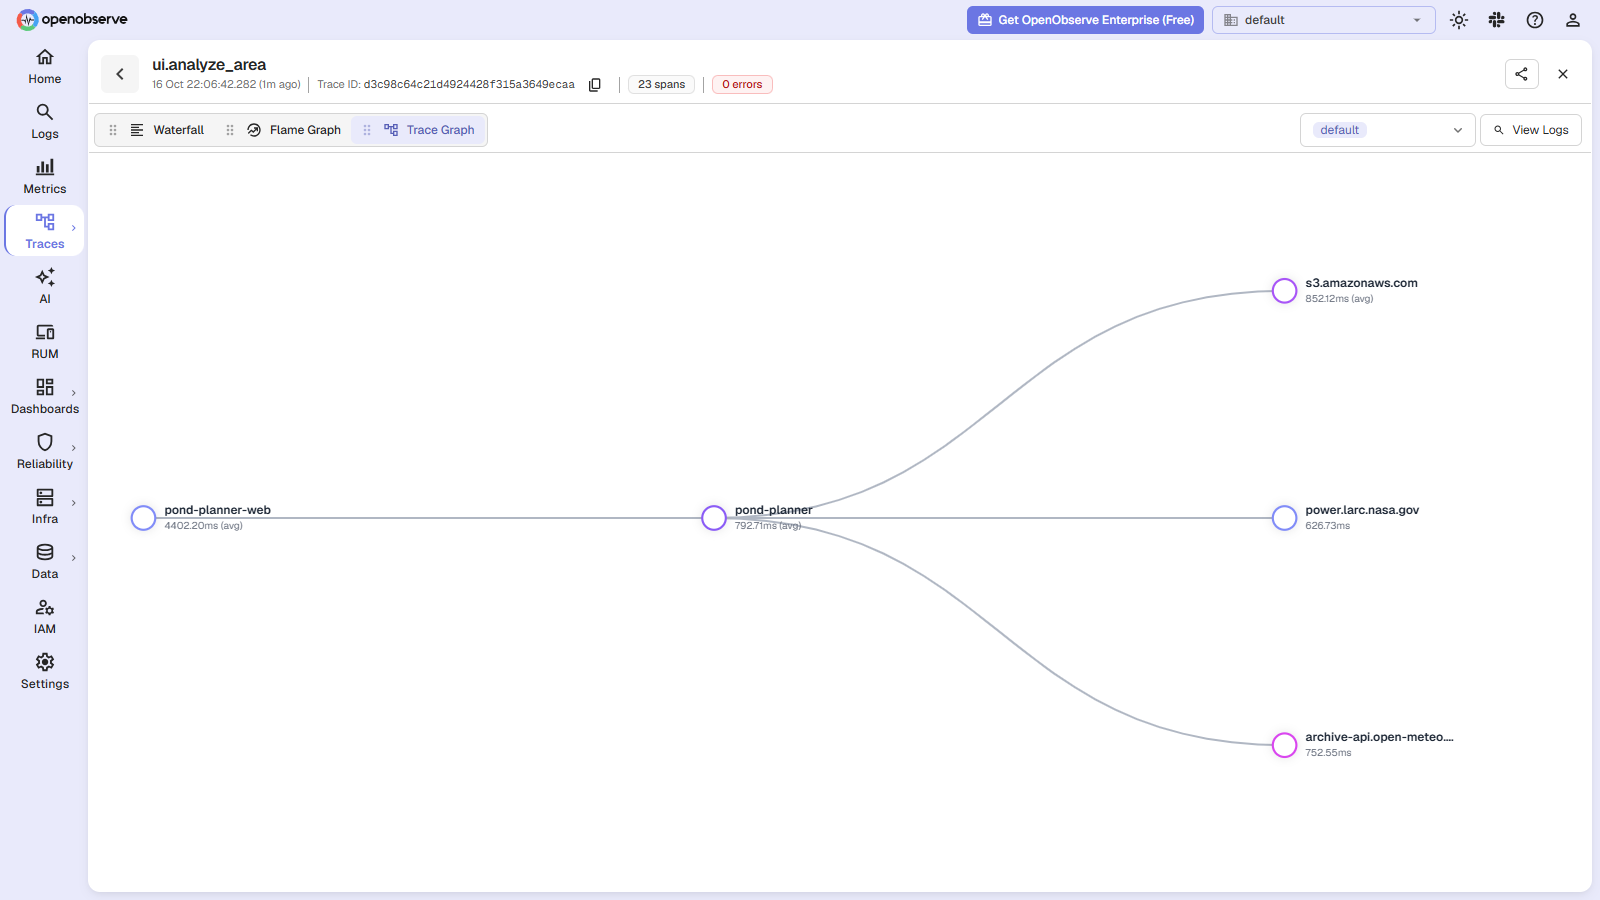
\includegraphics[width=0.85\linewidth]{figures/04_trace_graph}
  \caption{\textbf{Service graph of the same trace.} OpenObserve builds this
  from parent--child links alone: browser $\rightarrow$ backend
  $\rightarrow$ three external dependencies, with average latencies. We
  never drew this graph ourselves. It is the system's real dependency map,
  and it would show a new dependency if one appeared.}
  \label{fig:graph}
\end{figure}

\begin{figure}[htbp]
  \centering
  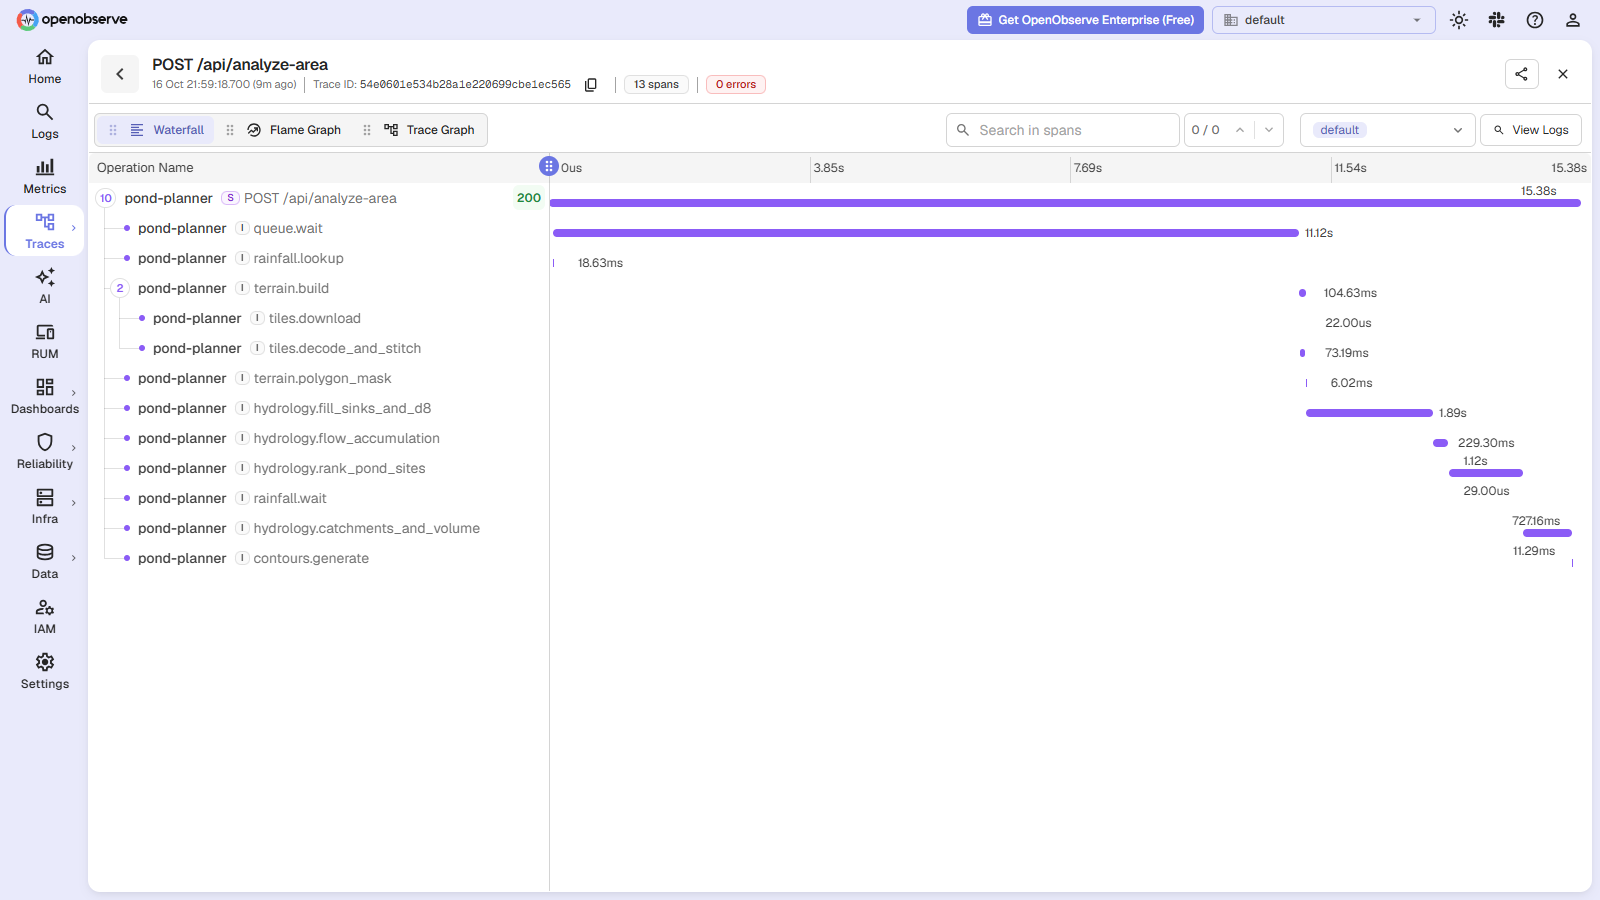
\includegraphics[width=\linewidth]{figures/05_trace_queue_wait}
  \caption{\textbf{Diagnosing a slow request.} Four users submitted 20~km$^2$
  areas at the same moment. The last one waited 15.4~s. Its trace shows
  that \textbf{11.1~s of that was \texttt{queue.wait}}: it was queued
  behind the other three, because the server runs one analysis at a time
  to stay within 1~vCPU and 512~MB. Its own work took about 4.2~s, the
  same as an unqueued request. Without the trace, this would look like
  ``the algorithm is slow on big areas''. With it, the answer is ``the
  algorithm is fine; we need more capacity or a smaller queue''. Tiles were
  cached, so \texttt{tiles.download} took 22~$\mu$s.}
  \label{fig:queue}
\end{figure}

\begin{figure}[htbp]
  \centering
  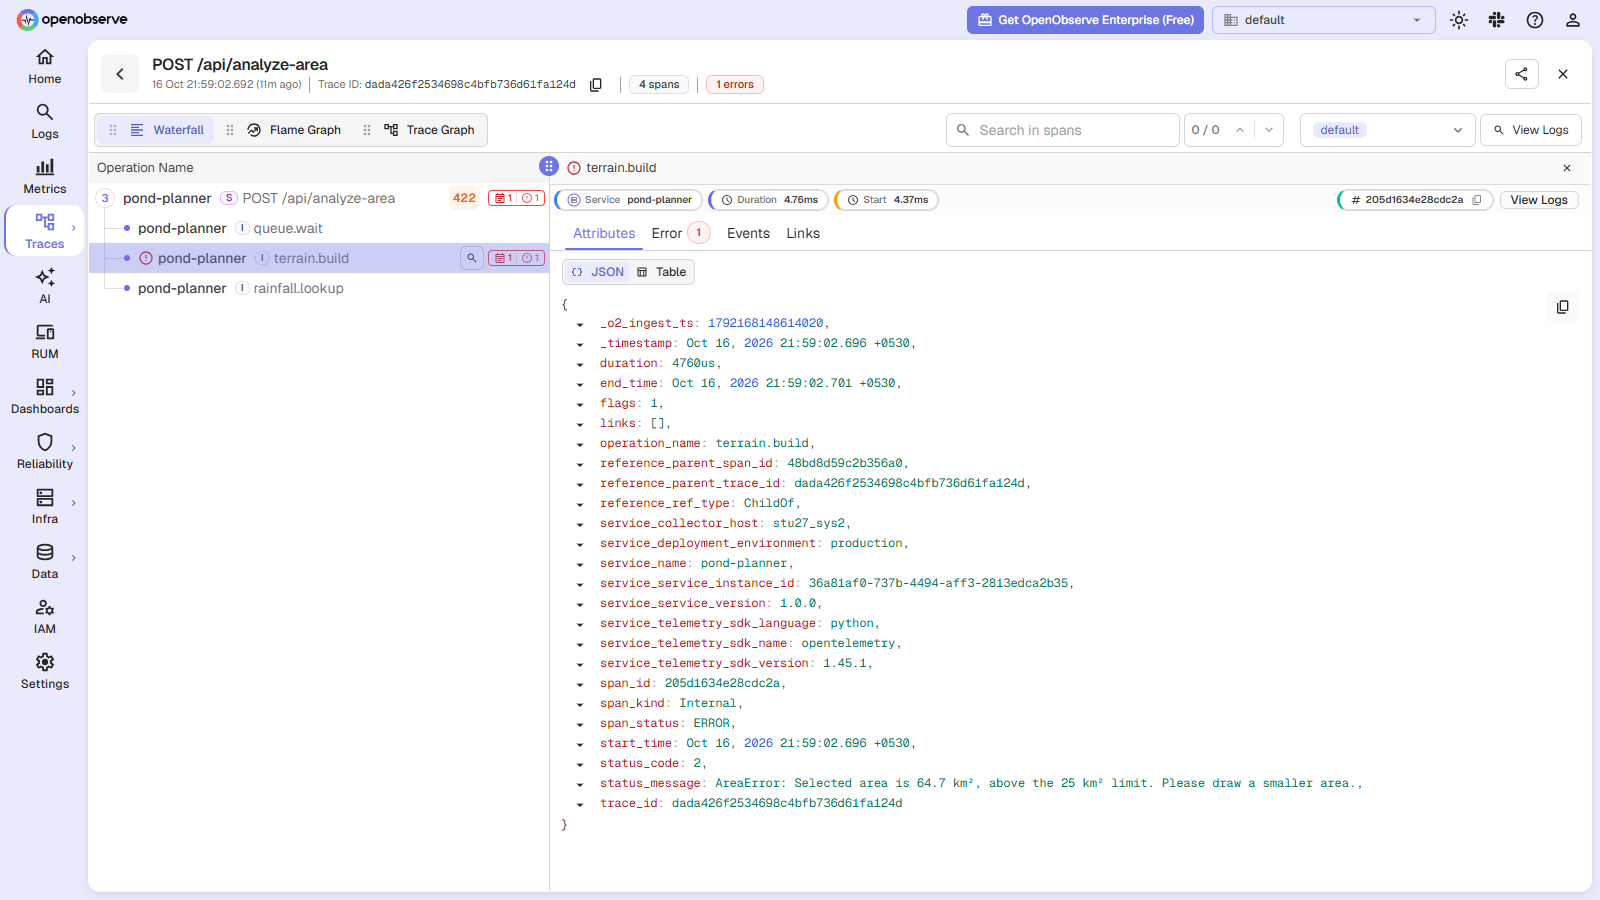
\includegraphics[width=\linewidth]{figures/06b_trace_rejected_exception}
  \caption{\textbf{An error, located.} A 64.7~km$^2$ request returned
  HTTP~422. The trace marks the exact span that failed
  (\texttt{terrain.build}, red icon, \texttt{span\_status: ERROR}). It
  records the exception message (``Selected area is 64.7~km$^2$, above the
  25~km$^2$ limit'') and shows the request was rejected 4.8~ms into
  terrain building, before any tile was downloaded. Users are told within
  milliseconds, and no work is wasted.}
  \label{fig:error}
\end{figure}

\begin{figure}[htbp]
  \centering
  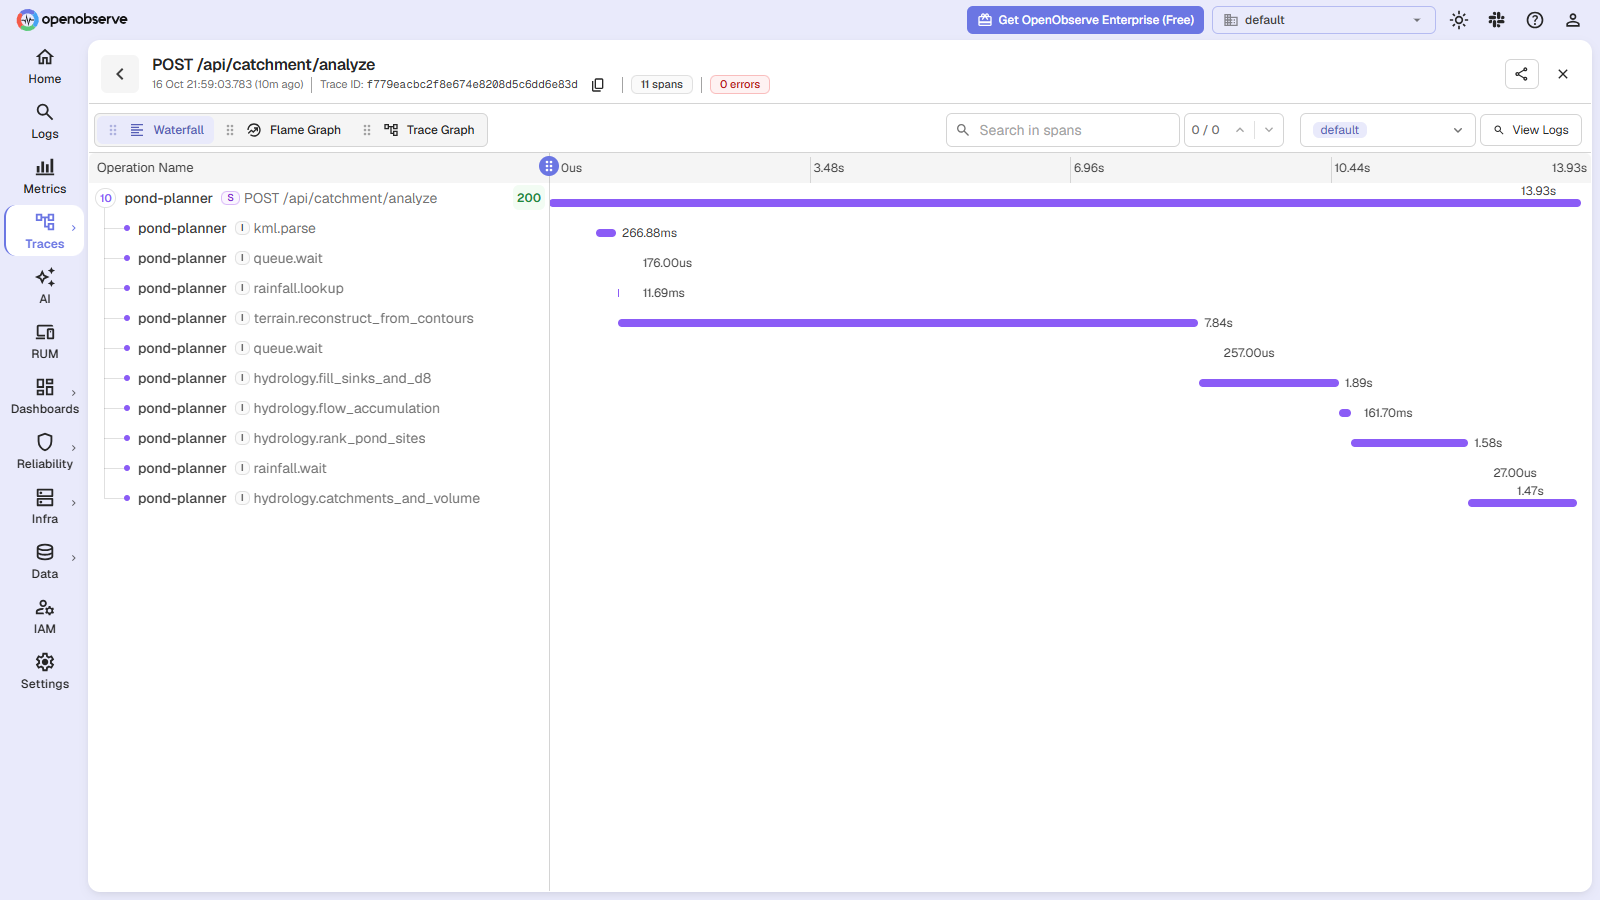
\includegraphics[width=\linewidth]{figures/07_trace_contour_upload}
  \caption{\textbf{The contour-upload path.} A 6.4~MB KML upload took
  13.9~s. Parsing took only 0.27~s. \texttt{terrain.reconstruct\_from\_contours}
  (interpolating contour lines into a grid) took \textbf{7.8~s, 56\% of the
  request}, more than all hydrology stages combined (5.1~s). If upload mode
  needs to be faster, interpolation is the place to optimise. Note the two
  \texttt{queue.wait} spans: the route takes the processing slot twice.}
  \label{fig:contour}
\end{figure}

\FloatBarrier
\subsection{Logs}

\begin{figure}[htbp]
  \centering
  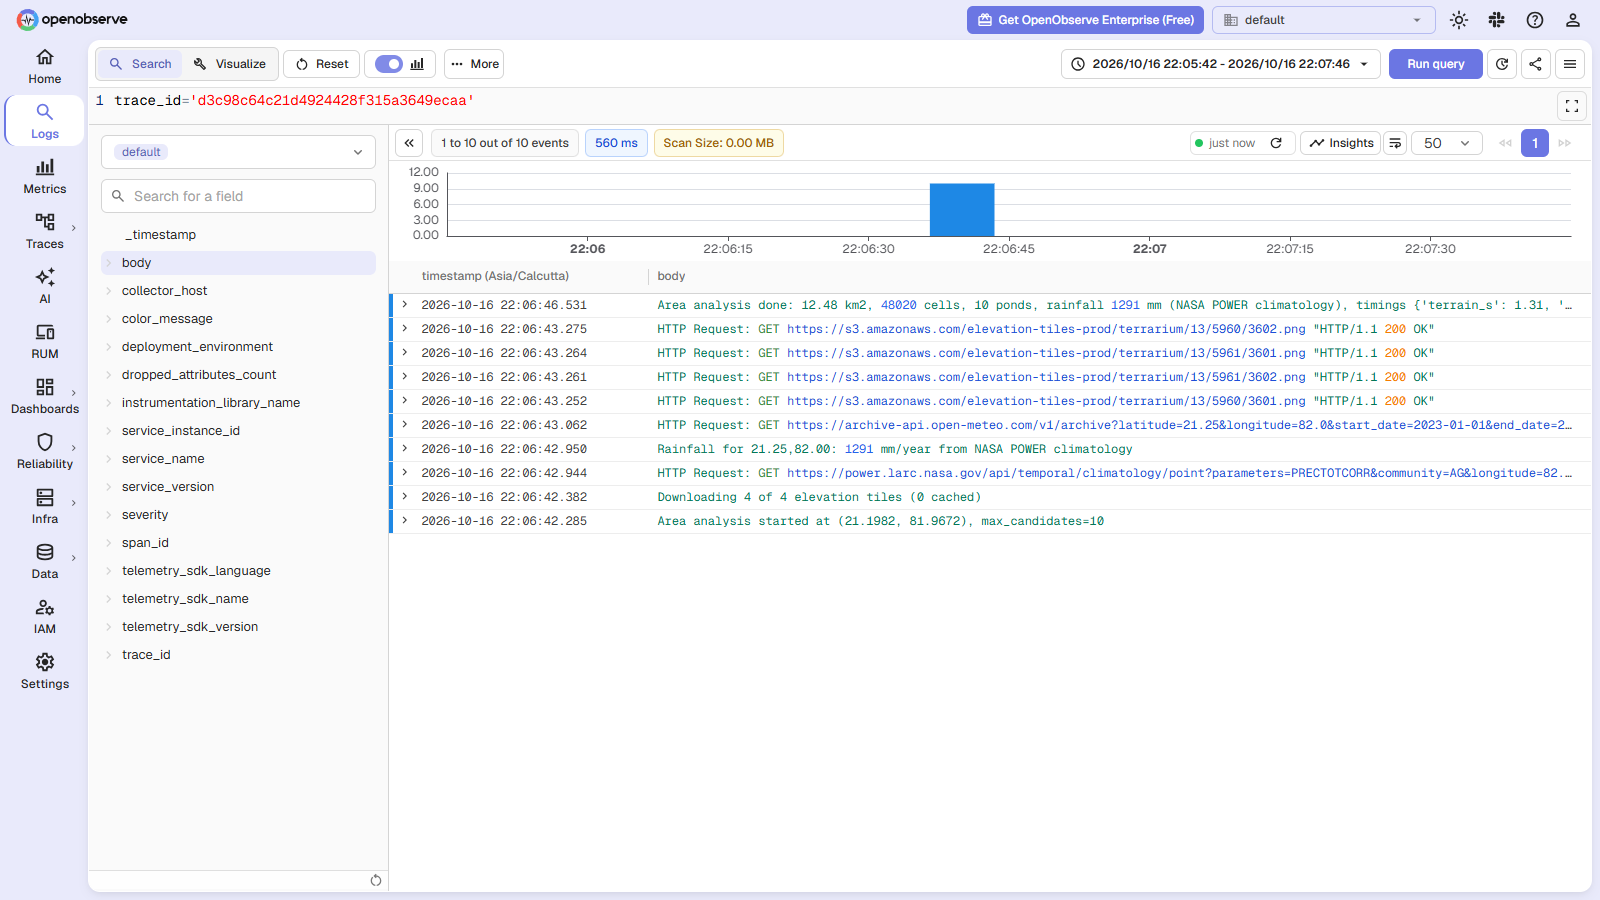
\includegraphics[width=\linewidth]{figures/08_logs_for_trace}
  \caption{\textbf{Logs correlated with a trace.} The \emph{View Logs}
  button on the trace in Figure~\ref{fig:waterfall} runs the query
  \texttt{trace\_id='d3c98c64\ldots'}. It returns exactly the ten log lines
  this request produced: the start and end of the analysis, ``Downloading
  4 of 4 elevation tiles (0 cached)'', each tile and rainfall HTTP call, and
  ``Rainfall for 21.25,82.00: 1291~mm/year from NASA POWER''. Before OpenTelemetry, these lines were interleaved with every other
  request's lines in \texttt{server.log}. Now one ID retrieves them.}
  \label{fig:logs-trace}
\end{figure}

\begin{figure}[htbp]
  \centering
  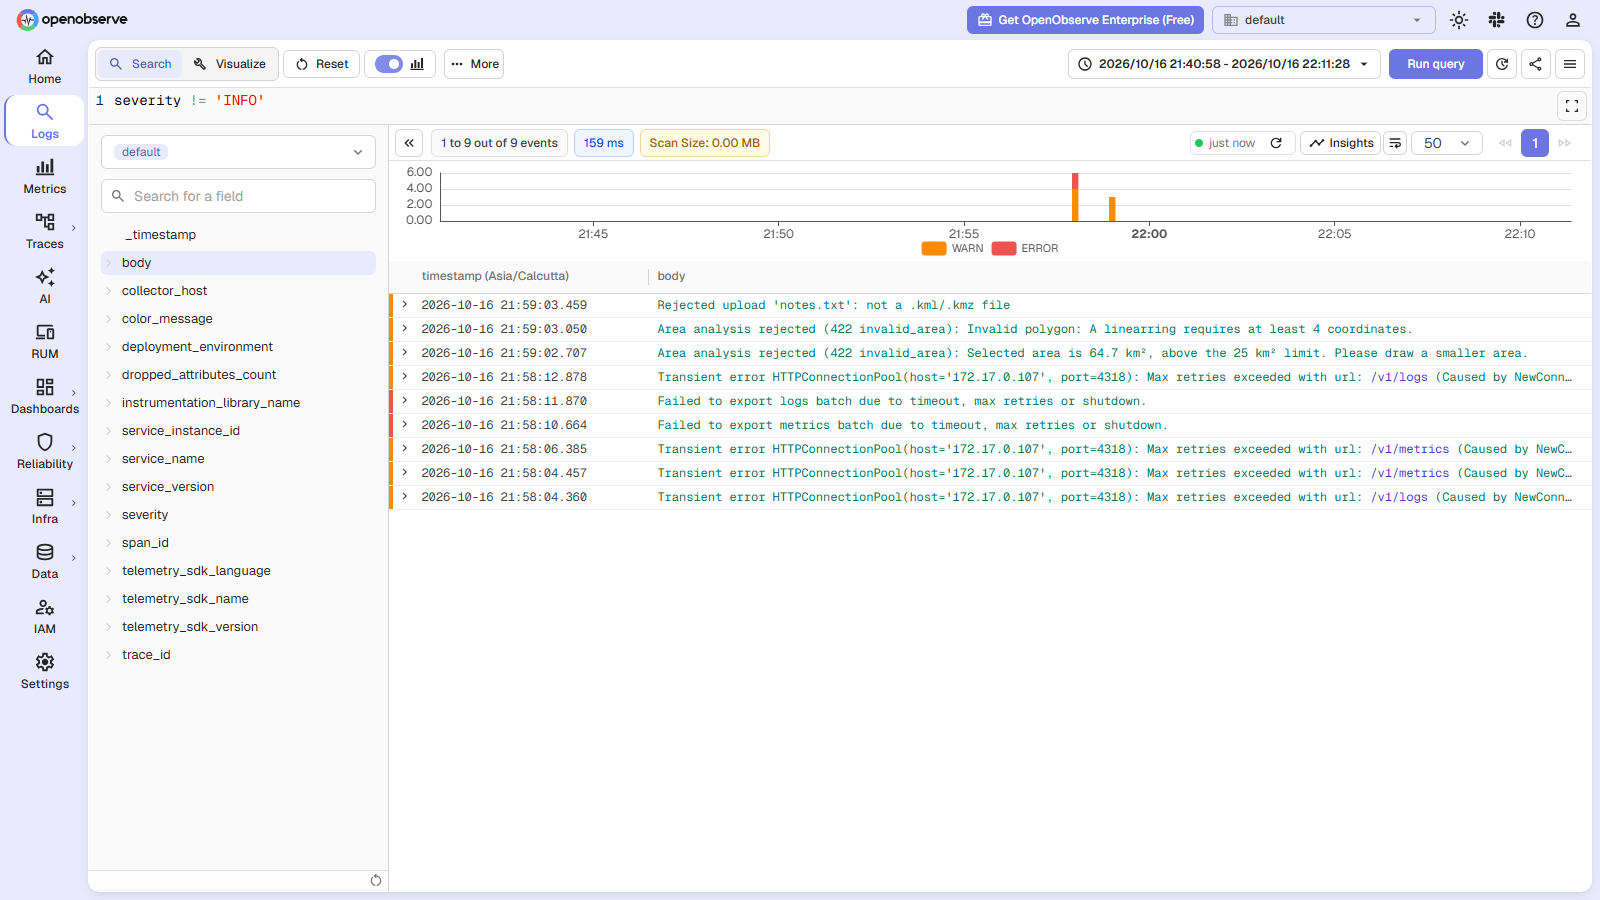
\includegraphics[width=\linewidth]{figures/09_logs_warnings_errors}
  \caption{\textbf{All warnings and errors} (\texttt{severity != 'INFO'}),
  coloured by level on the histogram. The three most recent lines are
  expected rejections: an invalid polygon, an over-limit area and a
  \texttt{.txt} upload. The six lines from 21:58 are more interesting. They
  are the OpenTelemetry SDK reporting that it \emph{could not reach the
  Collector} (``Connection refused'' on port 4318, then ``Failed to export
  metrics batch'') while we restarted the observability container.
  Telemetry recorded its own outage, and delivered that record once the
  Collector returned.}
  \label{fig:logs-errors}
\end{figure}

\FloatBarrier
\subsection{Metrics}

\begin{figure}[htbp]
  \centering
  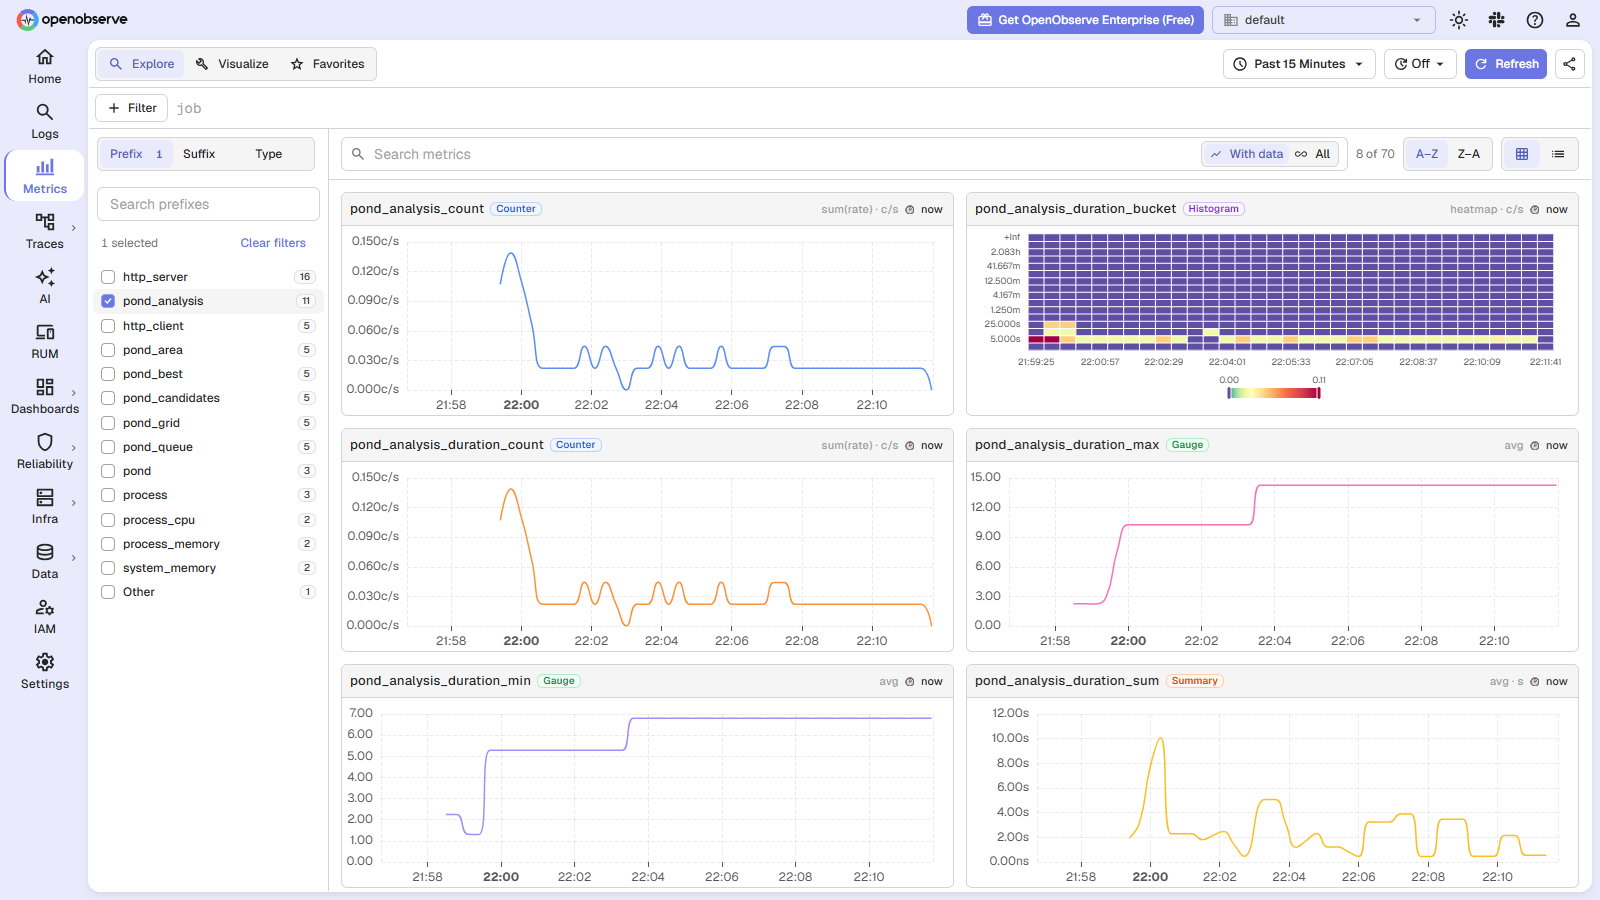
\includegraphics[width=\linewidth]{figures/10_metrics_pond_analysis}
  \caption{\textbf{Custom analysis metrics} (OpenObserve metrics explorer,
  prefix \texttt{pond\_analysis}). The rate of
  \texttt{pond\_analysis\_count} shows the scripted burst at 22:00 and then
  the slower background load. The duration histogram
  (\texttt{\_bucket}, heat map) shows how analysis times are distributed,
  not just their average. \texttt{\_max} steps up to 15~s when the four
  simultaneous requests arrived. As the lecture said, a metric tells you
  \emph{that} something changed, here at 22:00; the trace in
  Figure~\ref{fig:queue} tells you \emph{why}.}
  \label{fig:metrics-analysis}
\end{figure}

\begin{figure}[htbp]
  \centering
  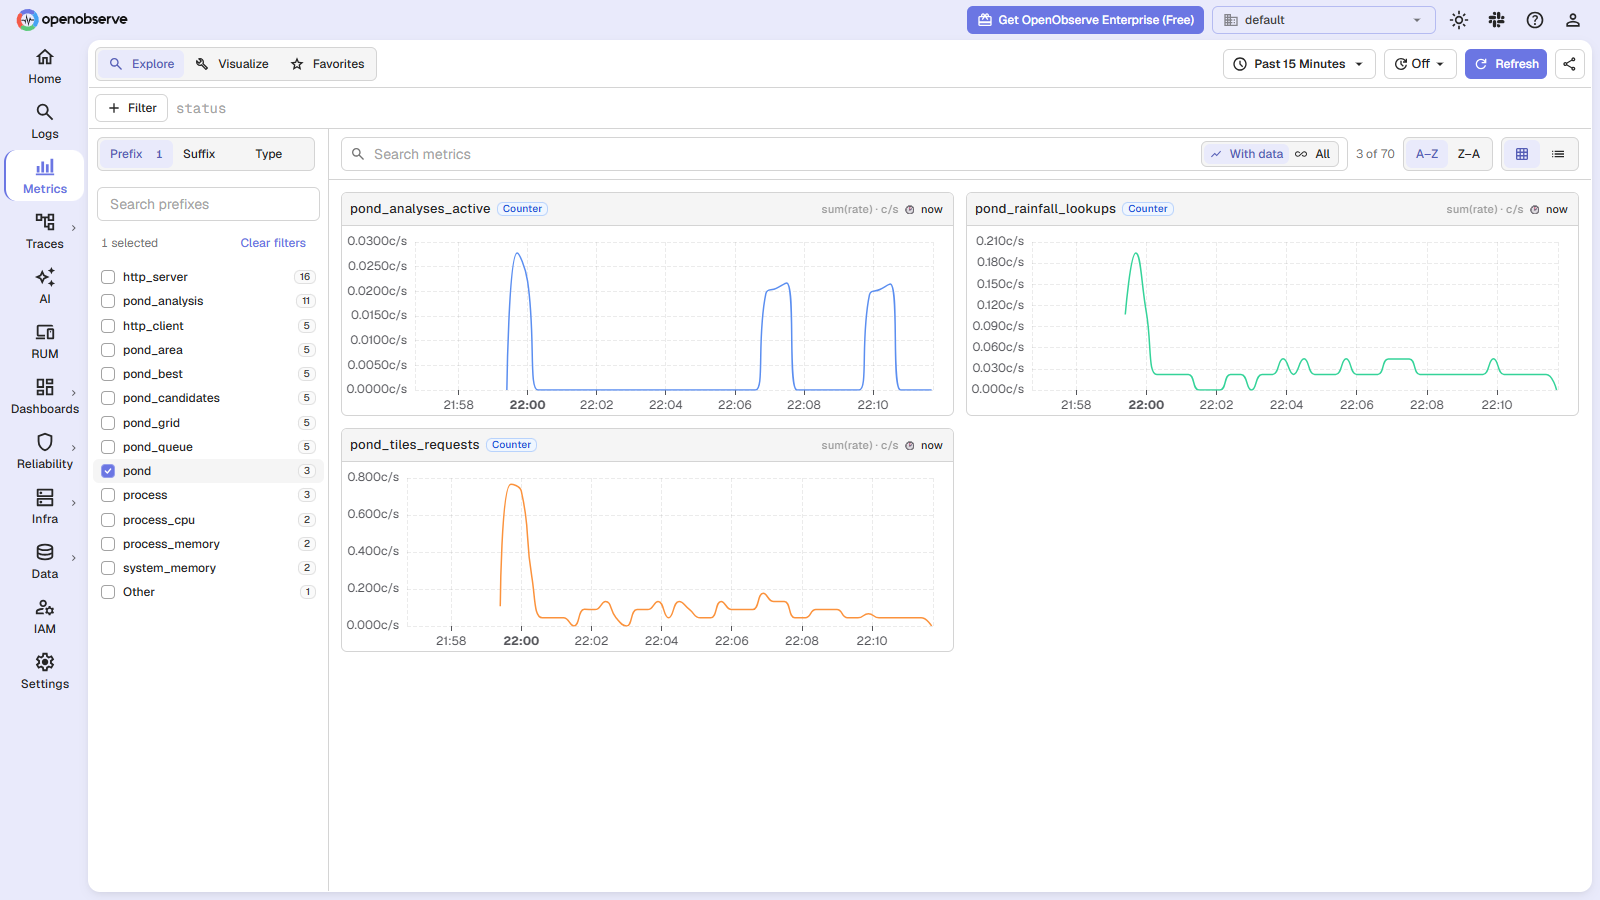
\includegraphics[width=\linewidth]{figures/11_metrics_pond_counters}
  \caption{\textbf{Supporting counters:} \texttt{pond\_analyses\_active} (work in
  progress or queued), \texttt{pond\_rainfall\_lookups} (lookups by the
  source that answered) and \texttt{pond\_tiles\_requests} (tiles needed
  per second, mostly cache hits after the first burst). Over the session, 61 tile requests were served from cache and 33 were
  downloaded. Cold \texttt{tiles.download} spans averaged 1.12~s; warm ones
  took under 1~ms.}
  \label{fig:metrics-counters}
\end{figure}

\begin{figure}[htbp]
  \centering
  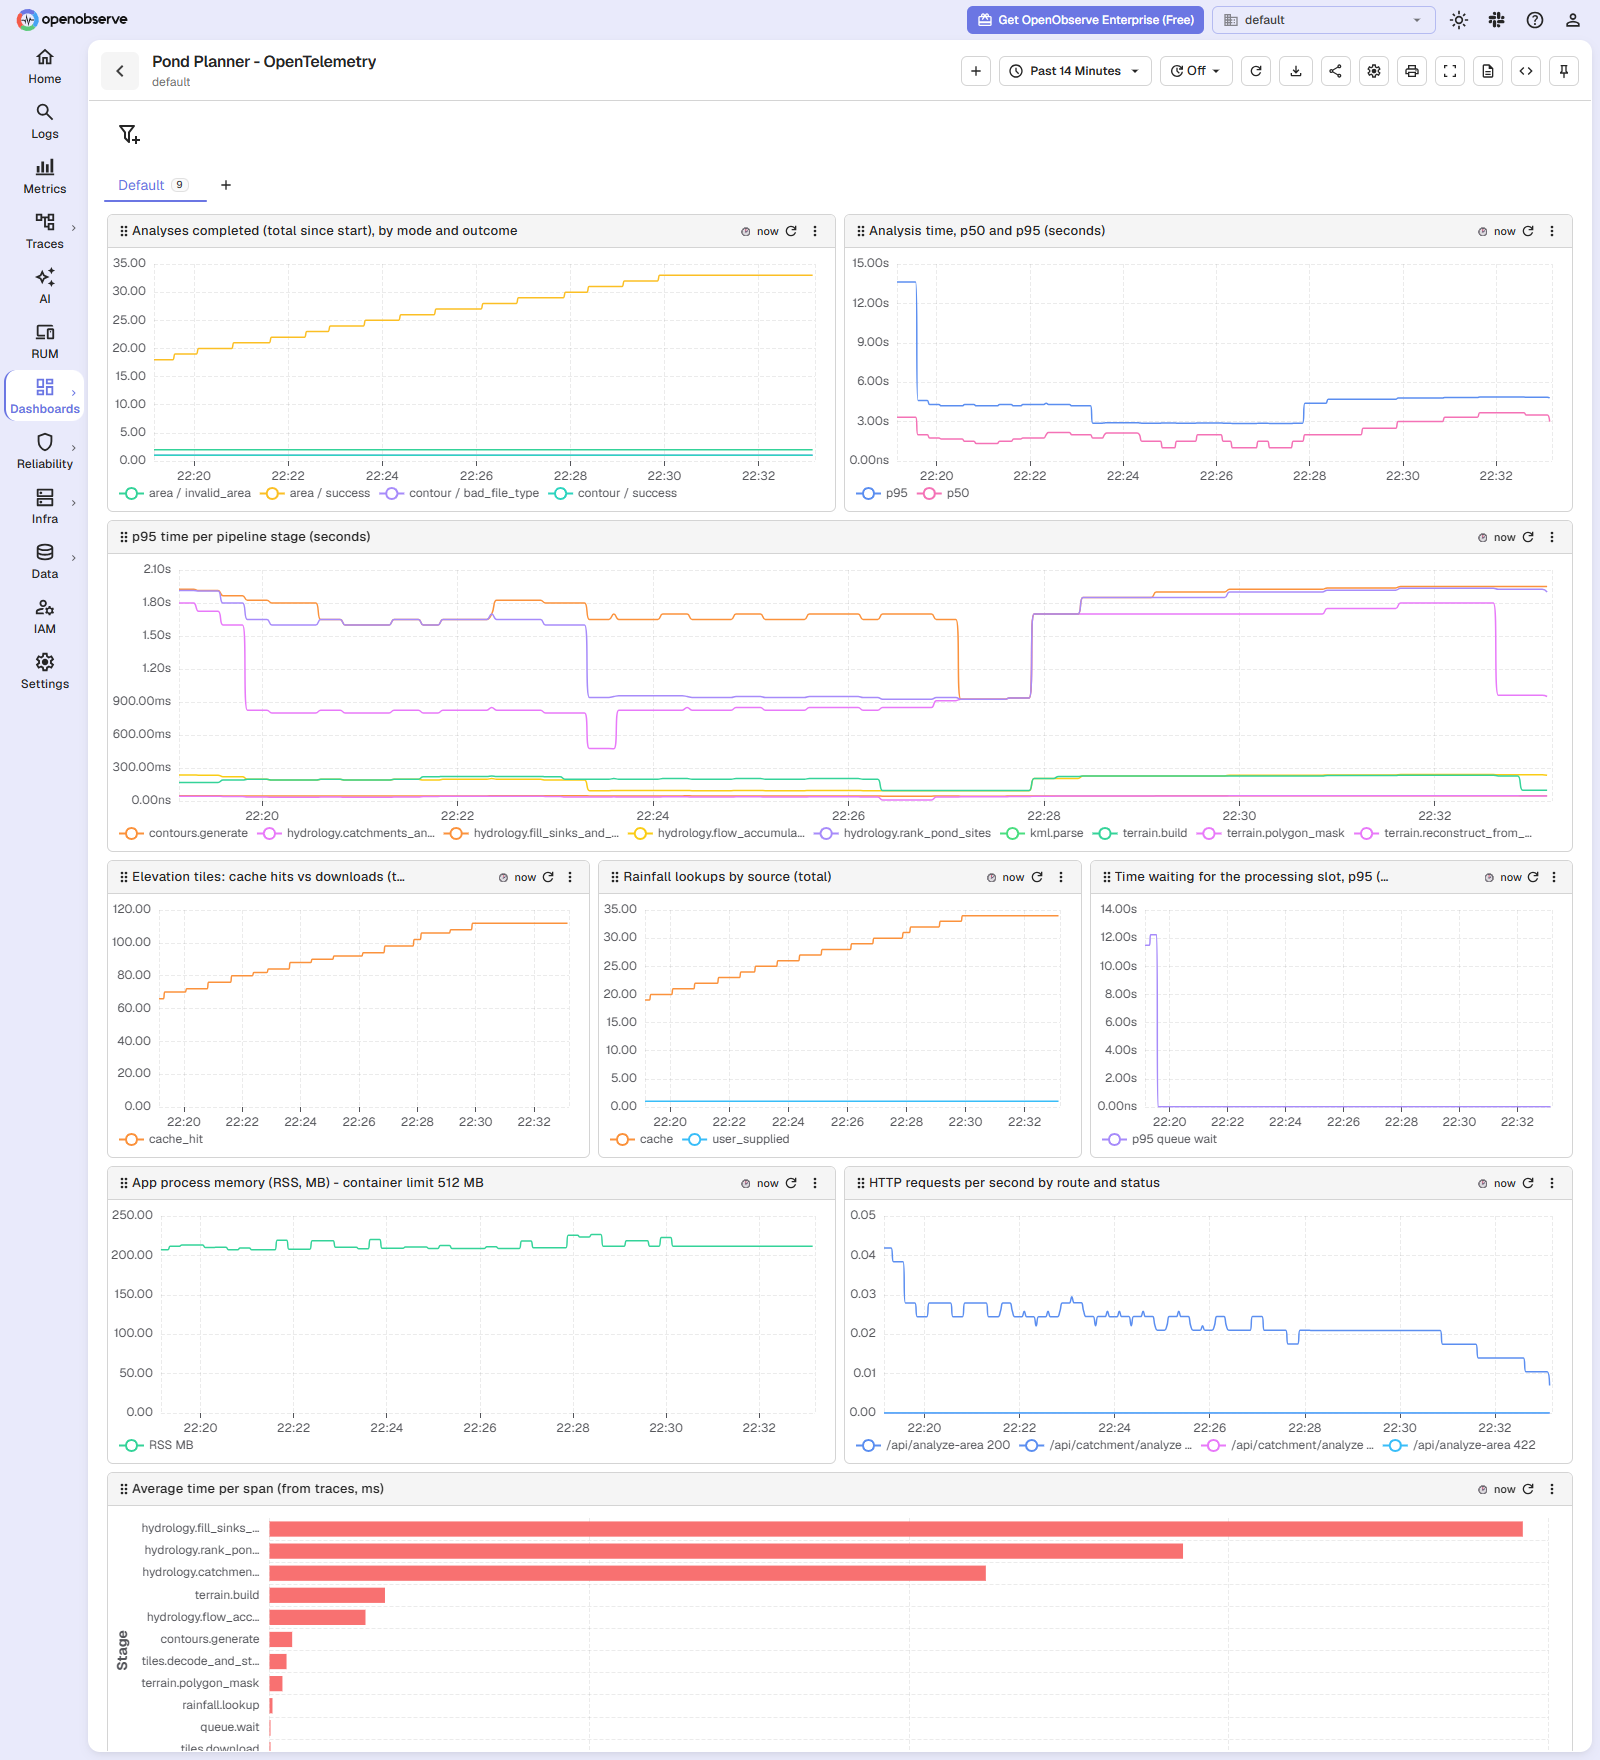
\includegraphics[width=\linewidth]{figures/14_dashboard}
  \caption{\textbf{Dashboard} built in OpenObserve from PromQL and SQL
  queries over the same data: analyses by outcome, p50 and p95 analysis
  time, p95 per pipeline stage, tile cache hits vs.\ downloads, rainfall
  source, queue wait, app memory against the 512~MB limit, HTTP rate by
  route and status, and average span duration taken from the traces. The
  window is the last 14 minutes of background load, after the histogram
  fix. Median analysis time is about 2~s and p95 about 4~s. The queue-wait
  panel shows the four-request burst (p95 12~s) and then zero. App memory
  holds near 210~MB, well inside the 512~MB limit. Every tile and rainfall
  lookup in this window was served from cache. Sink filling and D8 is the
  most expensive stage on average, followed by site ranking.}
  \label{fig:dashboard}
\end{figure}

\clearpage
%% =====================================================================
\section{What the data taught us}
\label{sec:lessons}

\paragraph{Where the time actually goes.} Averaged over 56 traced area
analyses, the backend stages ranked:
\begin{itemize}
\item \texttt{hydrology.fill\_sinks\_and\_d8}: 927~ms;
\item \texttt{tiles.download}: 681~ms, but only on a cold cache, and about
  0~ms warm;
\item \texttt{hydrology.rank\_pond\_sites}: 620~ms;
\item \texttt{hydrology.catchments\_and\_volume}: 492~ms.
\end{itemize}
In Assignment~1 we assumed downloads dominated and optimised them (async
client, caching). The traces confirm that this worked: on a warm cache,
the remaining cost is pure CPU work in sink filling and ranking. Those are
the next optimisation targets.

\paragraph{Racing two rainfall sources was justified.} Every lookup queries
NASA POWER and Open-Meteo at once and keeps the first answer. NASA won 30
races and Open-Meteo 26, so neither source is reliably faster. In one local
test, NASA's connection was reset and Open-Meteo answered alone. The
\texttt{rainfall.nasa\_power} span recorded the exception, and the request
still succeeded. Without the spans, this design decision would have been a
guess.

\paragraph{The three signals answer different questions.} The lecture's
summary held exactly:
\begin{itemize}
\item the \emph{metric} (Figure~\ref{fig:metrics-analysis}) showed that
  maximum analysis time jumped to 15~s at 22:00;
\item the \emph{trace} (Figure~\ref{fig:queue}) showed it was queueing, not
  computation;
\item the \emph{log} (``Analysis waited 11.1~s for the processing slot'')
  recorded it in words, linked by the same trace ID.
\end{itemize}
None of the three alone would have been enough.

\paragraph{Observability helped debug the observability stack.} After the
first deployment, data stopped appearing in OpenObserve.
\begin{itemize}
\item The Collector's own log showed \texttt{Exporting failed. Will retry},
  and OpenObserve logged \texttt{MemoryTableOverflowError} with HTTP~503.
\item The cause: inside the container, both OpenObserve and the Collector
  see all 120 CPUs of the host machine, not the one vCPU the container is
  allowed (the Collector logged \texttt{NumCPU: 120}). OpenObserve sizes its
  in-memory buffer buckets and thread pools from the CPU count. Our most
  likely explanation is that the 32~MB buffer we had configured was spread
  over so many buckets that each overflowed almost at once.
\item The fix: one bucket, a 96~MB buffer, flushing to disk every 60~s,
  and thread pools sized for one CPU. For the Collector we set
  \texttt{GOMAXPROCS=1}.
\item Because the Collector buffers and retries, the app was never
  slowed, and the delayed data arrived after the fix.
\end{itemize}

\paragraph{Clock skew is real.} The browser's span starts about 110~ms
\emph{after} the backend span it caused, which is physically impossible.
The laptop's clock is about 110~ms ahead of the server's. Distributed
traces combine timestamps from different machines, so durations
\emph{within} one service are exact, but offsets \emph{between} services are
only as good as clock synchronisation.

\paragraph{Cost.} The app process ran at about 150--280~MB RSS with
telemetry enabled, within the earlier measured range, and requests took
the same time as before (warm 1~km$^2$: 0.4~s). On the observability host,
OpenObserve used 270--330~MB and the Collector 30--85~MB. Batching keeps
network overhead low: one export carried 536 metric data points every
15~s.

%% =====================================================================
\section{Limitations}
\begin{itemize}
\item All traces are kept (no sampling). This is fine at course scale; under
  real load, a sampler or the Collector's tail sampling would keep only
  slow and failed traces.
\item OpenObserve keeps data on the container's disk with no replication;
  losing the container loses the history.
\item The browser sends its spans through the app, so a user who never
  reaches the app produces no browser telemetry.
\item No alerts are configured yet. An obvious first one is p95
  \texttt{pond.queue.wait} $>$ 10~s, which would signal that one processing
  slot is no longer enough.
\end{itemize}

%% =====================================================================
\section{Conclusion}
OpenTelemetry turned the pond planner from a black box with an access log
into a system we can question. Every request now has one ID that links:
\begin{itemize}
\item the user's click;
\item every pipeline stage and external call;
\item its log lines;
\item the aggregate metrics it contributes to.
\end{itemize}
The instrumentation is vendor-neutral, which is what the lecture called
``instrument once, send anywhere'': the code contains no reference to
OpenObserve, and the backend can be changed in the Collector's
configuration alone. The questions it answered (queueing vs.\ computation,
cold vs.\ warm cost, which rainfall source wins, why data was being
dropped) were real ones, and their answers changed what we would do next.

\appendix
\section{Reproducing the set-up}
\begin{lstlisting}[language=bash]
# Observability container (stu27_sys2): binaries + config in ~/observability
./start.sh   # OpenObserve on :3000 (published as :3306), Collector on :4318

# App container (stu27_sys1): ~/pond
export OTEL_SERVICE_NAME=pond-planner
export OTEL_EXPORTER_OTLP_ENDPOINT=http://172.17.0.107:4318
venv/bin/uvicorn app.main:app --app-dir backend --host 0.0.0.0 --port 3000
\end{lstlisting}
Source: \texttt{backend/app/telemetry.py} (set-up and metrics),
\texttt{frontend/src/telemetry.js} (browser),
\texttt{backend/app/api/routes/otel\_proxy.py} (browser span forwarding),
\texttt{observability/otelcol-config.yaml}, \texttt{observability/start.sh},
\texttt{observability/run-app.sh}.

\end{document}
